% ============================================================================
%  5. KẾT QUẢ VÀ PHÂN TÍCH
% ============================================================================
\section{Kết quả và phân tích}
\label{sec:ket-qua}

\subsection{Kết quả tổng thể}

\begin{table}[H]
\centering
\caption{Chỉ số đánh giá tổng thể trên 120 câu hỏi ($k = 5$), kèm khoảng tin cậy 95\% (Wilson)}
\label{tab:tong-the}
\renewcommand{\arraystretch}{1.2}
\begin{tabularx}{\textwidth}{@{}l r c L@{}}
\toprule
\textbf{Chỉ số} & \textbf{Giá trị} & \textbf{KTC 95\%} & \textbf{Ghi chú} \\
\midrule
Độ chính xác phân lớp & 95,83\% & [90,6\% -- 98,2\%] & 115/120 câu vào đúng lớp \\
\textbf{Top-1}        & \textbf{76,67\%} & [68,3\% -- 83,3\%] & Cổng chỉ số trong CI chặn mọi thay đổi làm tụt dưới mức này \\
Top-3                 & 90,83\% & [84,3\% -- 94,8\%] & 109/120 câu \\
Top-5                 & 95,00\% & [89,5\% -- 97,7\%] & 6/120 câu không có đáp án trong 5 kết quả \\
MRR                   & 0,8384  & ---                & Đáp án đúng thường nằm ở hạng 1--2 \\
Precision (macro)     & 0,3373  & ---                & Trần toán học 0,3707 --- xem mục~\ref{sec:kiem-dinh} \\
Recall (macro)        & 0,9306  & ---                & --- \\
F1 (macro)            & 0,4399  & ---                & --- \\
Thời gian trả lời TB  & 6,2~ms  & ---                & Chạy hoàn toàn cục bộ, đo trên máy cá nhân \\
\bottomrule
\end{tabularx}
\end{table}

Khoảng tin cậy được đưa vào có chủ đích. Với cỡ mẫu 120 câu, Top-1 76,67\% thực chất nằm
trong khoảng [68,3\% -- 83,3\%]. Nghĩa là một thay đổi làm Top-1 nhích 1--2 điểm phần trăm thì
\emph{không} kết luận được là cải tiến --- nhóm ghi rõ điều này để không diễn giải quá số liệu
mình có.

\subsection{Kết quả theo lớp bài toán}

\begin{table}[H]
\centering
\caption{Chỉ số theo từng lớp bài toán, kèm KTC 95\% của Top-1}
\label{tab:theo-lop}
\renewcommand{\arraystretch}{1.2}
\begin{tabularx}{\textwidth}{@{}L r r r c r@{}}
\toprule
\textbf{Lớp bài toán} & \textbf{$n$} & \textbf{Phân lớp} & \textbf{Top-1} & \textbf{KTC 95\% Top-1} & \textbf{Top-5} \\
\midrule
P1 · Tra cứu khái niệm     & 20 & 95,0\%  & 85,0\% & [64\% -- 95\%] & 95,0\% \\
\rowcolor{orange!8}
P2 · Tra cứu quy định      & 20 & 95,0\%  & 55,0\% & [34\% -- 74\%] & 85,0\% \\
P3 · Tra cứu chế tài       & 40 & 97,5\%  & 85,0\% & [71\% -- 93\%] & 97,5\% \\
P4 · Tra cứu ngược         & 12 & 100,0\% & 66,7\% & [39\% -- 86\%] & 100,0\% \\
P5 · Suy diễn tình huống   & 15 & 86,7\%  & 86,7\% & [62\% -- 96\%] & 93,3\% \\
P6 · Tra cứu căn cứ        & 8  & 100,0\% & 87,5\% & [53\% -- 98\%] & 100,0\% \\
P7 · Tra cứu liên quan     & 5  & 100,0\% & 40,0\% & [12\% -- 77\%] & 100,0\% \\
\bottomrule
\end{tabularx}
\end{table}

\textbf{Nhận xét.}
\begin{itemize}
  \item \textbf{P2} chỉ đạt Top-1 55,0\% nhưng Top-5 lên 85,0\%, và là lớp duy nhất có cả
        khoảng tin cậy nằm dưới mức chung 76,67\% --- tức là điểm yếu có thật chứ không do cỡ
        mẫu. Nguyên nhân: các quy tắc giao thông có nhiều điều khoản gần nghĩa; đáp án đúng
        thường \emph{có} trong danh sách trả về, chỉ chưa được xếp đầu.
  \item \textbf{P7} chỉ đạt Top-1 40,0\% nhưng Top-5 đạt 100,0\%. Với $n = 5$, con số 40\%
        thực chất là 2/5 câu và khoảng tin cậy rộng tới [12\% -- 77\%], nên gần như không kết
        luận được gì. Về bản chất, lớp ``tra cứu liên quan'' không có một đáp án duy nhất:
        người hỏi muốn một chùm tri thức, nên Top-5 mới là thước đo phù hợp.
  \item \textbf{P4} phân lớp đúng 100\% và Top-5 đạt 100\%, nhưng Top-1 chỉ 66,7\%: tra ngược
        theo mức phạt thường có nhiều hành vi cùng thoả điều kiện, và hệ thống trả về nguyên
        một \emph{tập} thoả ràng buộc, nên ``hạng 1'' ở lớp này là khái niệm ít ý nghĩa.
  \item \textbf{Câu nhiều đáp án chuẩn:} hệ lấy đủ toàn bộ đáp án ở 20/26 câu (76,92\%).
        Riêng lớp P4 đạt tuyệt đối; \textbf{P5 là nơi còn sót}: Top-5 tính là đúng chỉ cần
        tìm được \emph{một} vi phạm, nhưng muốn tính \emph{tổng} mức phạt thì phải tìm đủ
        mọi vi phạm --- điều này mới đạt 9/15 câu (60\%).
\end{itemize}

\subsection{Kiểm định ý nghĩa thống kê}
\label{sec:kiem-dinh}

Bốn kiểm định dưới đây trả lời bốn câu hỏi mà một bảng chỉ số đơn thuần không trả lời được.
Tất cả sinh ra từ \code{eval/kiem\_dinh.py}.

\subsubsection{Suy diễn số học có thật sự cải thiện, hay chỉ là may rủi?}

Kiểm định McNemar trên cùng bộ câu hỏi, so cấu hình C (lai ba thành phần) với cấu hình D
(thêm suy diễn số học): \textbf{12 câu} chuyển từ sai sang đúng, \textbf{0 câu} chuyển ngược
lại, $p = 0{,}000488$. Với $p < 0{,}001$, cải thiện này không phải ngẫu nhiên. Đáng chú ý hơn
cả trị số $p$ là hình dạng bảng chéo: không có câu nào bị suy diễn số học làm hỏng, nghĩa là
thành phần này chỉ thêm chứ không phá.

\subsubsection{Precision 0,3373 là kém hay đã kịch trần?}

Vì hệ trả $k = 5$ kết quả trong khi 94/120 câu chỉ có một mẩu tri thức đúng, precision của
những câu đó tối đa là $1/5 = 0{,}20$. Tính trần cho từng câu,
$P_i^{\max} = \min(|G_i|, |T_i|)/|T_i|$, rồi lấy trung bình được \textbf{0,3707}. Giá trị đo
được 0,3373 tương đương \textbf{91,0\%} của trần đó. Kết luận: precision thấp là hệ quả của
thiết kế top-$k$, không phải khiếm khuyết của mô hình --- và recall macro 0,9306 mới là chỉ số
phản ánh đúng mục tiêu của một hệ tra cứu.

\subsubsection{Hệ có chịu được truy vấn gõ không dấu?}

Chạy lại toàn bộ bộ câu hỏi sau khi bỏ dấu tiếng Việt: Top-1 76,67\%, Top-5 95,00\%, phân lớp
95,83\% --- \textbf{trùng khớp tuyệt đối} với bản có dấu ở cả bảy lớp bài toán. Có hai cơ chế
cùng bảo đảm điều này: (i) mọi keyphrase đều lưu kèm bản không dấu và B1 chuẩn hoá về bản đó;
(ii) hai bộ nhận dạng cấu trúc --- căn cứ điều khoản và ràng buộc số --- có bộ mẫu riêng cho
câu gõ không dấu.

\begin{warnbox}
Cơ chế (ii) là kết quả của chính phép kiểm định này. Ở phiên bản trước, bộ nhận dạng chỉ dò mẫu
có dấu nên khi bỏ dấu, lớp P6 rơi từ 7/8 xuống 0/8 và P4 từ 8/12 xuống 3/12 (Top-1 tổng còn
66,67\%). Lỗi đã được sửa và khoá bằng 24 test; bộ mẫu không dấu cố ý chặt hơn, vì mất dấu thì
``đèn'' và ``đến'', ``tự'' và ``từ'' trùng mặt chữ. Chỉ số trên câu có dấu không đổi một chữ số
nào sau khi sửa.
\end{warnbox}

\subsubsection{Mọi câu hỏi có thật sự chấm được?}

Có test kiểm chứng rằng toàn bộ 120/120 câu đều có đáp án chuẩn giải được về tri thức
\emph{có thật} trong cơ sở tri thức, không định danh treo nào. Nếu bước này không được kiểm,
mọi chỉ số ở trên đều vô nghĩa vì hệ thống có thể đang bị chấm trên những câu không thể đúng.

\subsection{Thí nghiệm loại bỏ thành phần}
\label{sec:ablation}

Để chứng minh từng thành phần của hàm điểm thực sự đóng góp chứ không phải chọn trọng số cảm
tính, nhóm chạy thí nghiệm loại bỏ thành phần trên cả 120 câu hỏi.

\begin{table}[H]
\centering
\caption{Kết quả loại bỏ thành phần (ablation) trên 120 câu hỏi}
\label{tab:ablation}
\renewcommand{\arraystretch}{1.2}
\begin{tabularx}{\textwidth}{@{}L r r r@{}}
\toprule
\textbf{Cấu hình} & \textbf{Top-1} & \textbf{Top-5} & \textbf{MRR} \\
\midrule
A. Chỉ so khớp ngữ nghĩa (TF-IDF)          & 58,3\% & 89,2\% & 0,7054 \\
B. Chỉ so khớp keyphrase                   & 35,8\% & 59,2\% & 0,4381 \\
C. Lai keyphrase + ngữ nghĩa + ngữ cảnh    & 66,7\% & 94,2\% & 0,7759 \\
\textbf{D. Hệ thống đầy đủ (C + suy diễn số học)} & \textbf{76,7\%} & \textbf{95,0\%} & \textbf{0,8384} \\
\bottomrule
\end{tabularx}
\end{table}

\begin{table}[H]
\centering
\caption{Ablation riêng trên 22 câu hỏi có giá trị số (nồng độ cồn, tốc độ)}
\label{tab:ablation-so}
\renewcommand{\arraystretch}{1.2}
\begin{tabularx}{\textwidth}{@{}L r r r@{}}
\toprule
\textbf{Cấu hình} & \textbf{Top-1} & \textbf{Top-5} & \textbf{MRR} \\
\midrule
C. Lai keyphrase + ngữ nghĩa + ngữ cảnh          & 40,9\% & 95,5\%  & 0,6364 \\
\textbf{D. Hệ thống đầy đủ (C + suy diễn số học)} & \textbf{95,5\%} & \textbf{100,0\%} & \textbf{0,9773} \\
\bottomrule
\end{tabularx}
\end{table}

\textbf{Nhận xét.}
\begin{itemize}
  \item Keyphrase đứng riêng (35,8\%) \emph{yếu hơn} TF-IDF đứng riêng (58,3\%), nhưng vẫn xứng
        đáng nhận trọng số cao nhất 0,55. Lý do: nó thua về \textbf{độ phủ} chứ không thua về
        \textbf{độ chính xác} --- câu nào có keyphrase thì gần như chắc đúng, chỉ là nhiều câu
        khẩu ngữ không có keyphrase nào.
  \item Lai ba thành phần đưa Top-1 lên 66,7\%: TF-IDF lo phần phủ, keyphrase lo phần chuẩn.
        Hai tín hiệu bù trừ nhau chứ không trùng lặp.
  \item Thêm suy diễn số học đưa Top-1 lên 76,7\%. Riêng 22 câu có giá trị số, Top-1 nhảy từ
        40,9\% lên 95,5\% trong khi Top-5 gần như không đổi. So khớp từ khoá \emph{vẫn tìm ra}
        đủ các khung phạt, nó chỉ không biết \emph{chọn khung nào}; suy diễn số học giải quyết
        đúng khâu đó, và cải thiện này có ý nghĩa thống kê ($p = 0{,}000488$).
  \item Lưu ý kỹ thuật: cấu hình C chỉ tắt \emph{bảng tra theo đại lượng} của bộ suy diễn số
        học, phần so ngưỡng vẫn chạy. Vì vậy mức tăng 10 điểm là \emph{cận dưới} của đóng góp
        thật.
\end{itemize}

\subsection{Phân tích lỗi sâu}

Thay vì chỉ liệt kê câu sai, nhóm chạy lại toàn bộ bộ câu hỏi, ghi \emph{hạng} của đáp án chuẩn
trong danh sách trả về, rồi quy mỗi ca chưa tối ưu về một nguyên nhân gốc duy nhất theo thứ tự
ưu tiên. Kết quả: \textbf{31/120 ca chưa tối ưu}. Trong đó chỉ 6 ca đáp án rơi hẳn ngoài
Top-5; 22 ca đáp án \emph{vẫn} nằm trong danh sách trả về nhưng không đứng đầu; 3 ca đáp án đã
ở hạng 1 nhưng câu hỏi bị gán sai lớp bài toán. Nói cách khác, phần lớn cái gọi là ``lỗi'' ở đây
là lỗi \textbf{xếp hạng}, không phải lỗi tìm kiếm.

\begin{table}[H]
\centering
\caption{Sáu nhóm nguyên nhân gốc và số ca}
\label{tab:nguyen-nhan}
\renewcommand{\arraystretch}{1.2}
\begin{tabularx}{\textwidth}{@{}c L r c@{}}
\toprule
\textbf{Mã} & \textbf{Nguyên nhân gốc} & \textbf{Số ca} & \textbf{Mức độ} \\
\midrule
L5 & Khoảng trống từ vựng làm tụt hạng        & 15 & Vừa \\
L1 & Định tuyến sai lớp bài toán              & 5  & Nặng \\
L3 & Thứ tự trong tập trả về (P4/P6/P7)       & 5  & Nhẹ \\
L2 & Trượt hẳn ngoài Top-$k$                  & 4  & Nặng \\
L4 & Câu nhiều đáp án chuẩn                   & 1  & Nhẹ \\
L6 & Khác                                     & 1  & Vừa \\
\midrule
   & \textbf{Tổng}                            & \textbf{31} & \\
\bottomrule
\end{tabularx}
\end{table}

\begin{figure}[H]
\centering
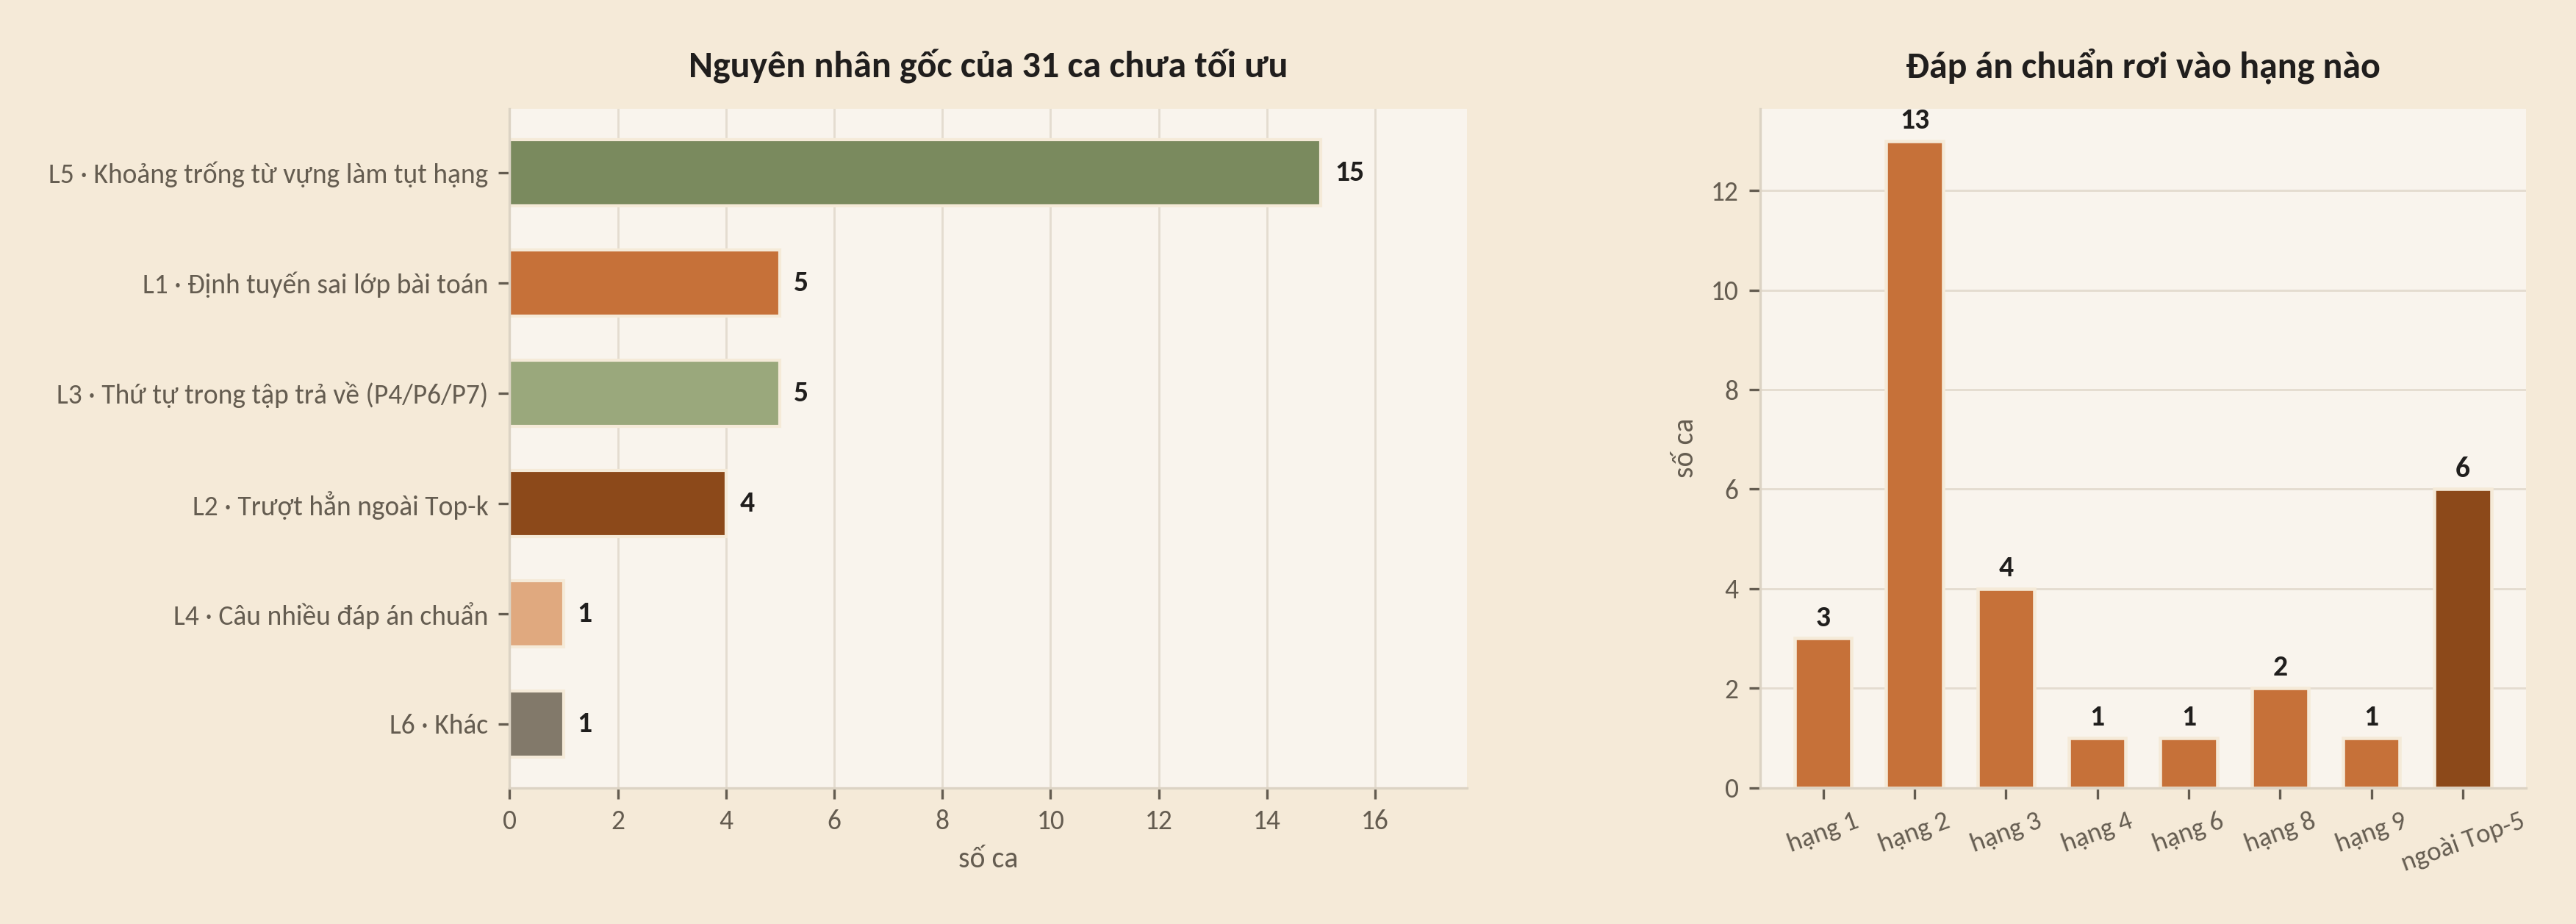
\includegraphics[width=\textwidth]{figures/hinh6_phan_tich_loi.png}
\caption{Phân tích lỗi sâu --- nguyên nhân gốc và hạng của đáp án chuẩn}
\label{fig:loi}
\end{figure}

\textbf{Diễn giải từng nhóm.}
\begin{itemize}
  \item \textbf{L5 --- Khoảng trống từ vựng} (15 ca, nhóm lớn nhất). Câu hỏi dùng từ đời thường
        không xuất hiện trong bất kỳ cụm từ khoá nào của đáp án: ``nón bảo hiểm'' thay vì ``mũ
        bảo hiểm'', ``bằng lái'' thay vì ``giấy phép lái xe''. Làn keyphrase im lặng, chỉ còn
        TF-IDF gánh, nên đáp án tụt xuống hạng 2--3 chứ hiếm khi rơi hẳn. Đây là lỗi sửa được
        bằng \emph{dữ liệu} (bổ sung biến thể khẩu ngữ), không cần đổi thuật giải.
  \item \textbf{L1 --- Định tuyến sai lớp} (5 ca, nặng nhất). Bước B3 chọn nhầm lớp nên bộ giải
        sai kiểu chạy. Ví dụ ``Đèn giao thông có mấy màu?'' bị đẩy sang P7 vì câu quá ngắn;
        ``Bằng lái bị trừ hết 12 điểm rồi thì sao\dots'' bị đẩy sang P4 vì con số 12 kích hoạt
        mẫu tra cứu ngược và nhận về danh sách rỗng.
  \item \textbf{L2 --- Trượt hẳn ngoài Top-5} (4 ca). Đây mới là lỗi người dùng thật sự cảm nhận
        được. Cả bốn ca đều là câu khẩu ngữ dài kể tình huống, hoặc câu dạng có/không (``Gặp đèn
        đỏ thì có được đi tiếp không?'') --- người hỏi chờ một câu khẳng định, hệ thống trả điều
        khoản gần nghĩa nhất.
  \item \textbf{L3 --- Thứ tự trong tập trả về} (5 ca, nhẹ nhất). Toàn bộ thuộc lớp P4/P6/P7,
        nơi hệ thống trả nguyên một tập thoả ràng buộc. Đáp án có trong tập, chỉ không đứng đầu
        --- đây là vấn đề trình bày chứ không phải truy hồi.
  \item \textbf{L4 và L6} (mỗi nhóm 1 ca). Hạng 1 là một mẩu tri thức cũng hợp lệ nhưng không
        trùng mẩu được chấm.
\end{itemize}

\begin{table}[H]
\centering
\caption{Một số ca tiêu biểu và nguyên nhân}
\label{tab:ca-tieu-bieu}
\small
\renewcommand{\arraystretch}{1.2}
\begin{tabularx}{\textwidth}{@{}c L c >{\raggedright\arraybackslash}p{4.3cm}@{}}
\toprule
\textbf{Mã} & \textbf{Câu hỏi} & \textbf{Hạng} & \textbf{Nguyên nhân} \\
\midrule
Q011 & Đèn giao thông có mấy màu? & 1 & L1 · Định tuyến sai lớp \\
Q020 & Mấy cái xe tự chạy không cần người lái ấy, trong luật gọi là gì\dots & ngoài Top-5 & L2 · Trượt ngoài Top-$k$ \\
Q021 & Gặp đèn đỏ thì có được đi tiếp không? & ngoài Top-5 & L2 · Trượt ngoài Top-$k$ \\
Q032 & Bằng lái bị trừ hết 12 điểm rồi thì sao, có được chạy xe nữa không\dots & ngoài Top-5 & L1 · Định tuyến sai lớp \\
Q035 & Chở con nhỏ trên ô tô thì luật quy định cháu ngồi ở đâu? & ngoài Top-5 & L2 · Trượt ngoài Top-$k$ \\
Q080 & Không chịu dừng xe khi cảnh sát giao thông ra hiệu kiểm tra thì\dots & ngoài Top-5 & L1 · Định tuyến sai lớp \\
Q096 & Nhóm em 4 đứa đi chung một xe máy, không ai đội mũ bảo hiểm\dots & 1 & L1 · Định tuyến sai lớp \\
Q101 & Xe ô tô của tôi bị che mất biển số và đã quá hạn đăng kiểm\dots & ngoài Top-5 & L2 · Trượt ngoài Top-$k$ \\
\bottomrule
\end{tabularx}
\end{table}

\subsection{Giải thích: vì sao các con số lại như vậy}

Bốn cơ chế dưới đây giải thích gần như toàn bộ hình dạng của kết quả.
\begin{enumerate}
  \item \textbf{Vì sao Top-5 (95,00\%) bỏ xa Top-1 (76,67\%)?} Vì cơ chế bổ sung tri thức không
        để bước phân lớp chặn kết quả: kể cả khi B3 chọn sai lớp, hệ vẫn nạp thêm tri thức của
        các loại còn thiếu nếu điểm vượt 0,40. Đáp án đúng hiếm khi biến mất khỏi danh sách,
        chỉ thường không đứng đầu --- đúng như 22 ca ở Bảng~\ref{tab:nguyen-nhan}.
  \item \textbf{Vì sao khoảng cách đó lớn nhất ở P2?} Quy tắc giao thông là loại tri thức có
        nhiều điều khoản gần nghĩa nhất --- nhường đường, chuyển hướng, quay đầu chia sẻ rất
        nhiều từ vựng. Cả ba làn điểm đều cho các ứng viên này số gần nhau, và hệ chưa có tín
        hiệu nào tách chúng ngoài độ tương đồng văn bản.
  \item \textbf{Vì sao suy diễn số học tạo khác biệt lớn (40,9\% $\to$ 95,5\%) mà Top-5 gần như
        không đổi?} Vì bài toán ở nhóm câu này không phải \emph{tìm} mà là \emph{chọn}. Các khung
        phạt của cùng một hành vi có văn bản gần như giống hệt nhau, chỉ khác con số ngưỡng; chỉ
        khi so sánh khoảng số mới chọn đúng được.
  \item \textbf{Vì sao hệ chưa từ chối được truy vấn ngoài lĩnh vực?} Vì đặc trưng TF-IDF mặc
        định không tách được hai phân bố: 56/120 câu hợp lệ chấm điểm thấp hơn hoặc bằng truy
        vấn rác, nên không tồn tại ngưỡng nào vừa loại hết rác vừa không từ chối oan
        (mục~\ref{sec:han-che}).
\end{enumerate}

\subsection{Kiểm thử nghiệm thu và kiểm thử tự động}

\begin{table}[H]
\centering
\caption{Mười hai ca nghiệm thu chức năng}
\label{tab:nghiem-thu}
\small
\renewcommand{\arraystretch}{1.18}
\begin{tabularx}{\textwidth}{@{}c >{\raggedright\arraybackslash}p{2.9cm} L c@{}}
\toprule
\textbf{Mã} & \textbf{Nhóm} & \textbf{Câu hỏi} & \textbf{Kết quả} \\
\midrule
TC01 & Lớp bài toán    & Xe cơ giới là gì? & \dat{} Đạt \\
TC02 & Lớp bài toán    & Người lái xe phải mang theo giấy tờ gì? & \dat{} Đạt \\
TC03 & Lớp bài toán    & Vượt đèn đỏ xe máy phạt bao nhiêu? & \dat{} Đạt \\
TC04 & Lớp bài toán    & Lỗi nào bị trừ 10 điểm giấy phép lái xe? & \dat{} Đạt \\
TC05 & Lớp bài toán    & Tôi vừa vượt đèn đỏ vừa không có giấy phép lái xe thì bị phạt bao nhiêu? & \dat{} Đạt \\
TC06 & Lớp bài toán    & Điều 6 khoản 9 điểm a Nghị định 168/2024/NĐ-CP nói về lỗi gì? & \dat{} Đạt \\
TC07 & Lớp bài toán    & Cho tôi thông tin về điểm của giấy phép lái xe. & \dat{} Đạt \\
TC08 & Suy diễn số học & xe máy nồng độ cồn 0,3 mg/l phạt bao nhiêu & \dat{} Đạt \\
TC09 & Suy diễn số học & ô tô nồng độ cồn 0,5 mg/l phạt bao nhiêu & \dat{} Đạt \\
TC10 & Ngữ nghĩa       & nhậu xong lái xe máy bị phạt nhiêu tiền\textsuperscript{a} & \dat{} Đạt \\
TC11 & Ngữ nghĩa       & khong doi mu bao hiem phat bao nhieu & \dat{} Đạt \\
TC12 & Ngữ nghĩa       & chạy quá tốc độ 25 km/h thì sao & \dat{} Đạt \\
\bottomrule
\multicolumn{4}{@{}p{\textwidth}@{}}{\footnotesize\textsuperscript{a}\,Chữ ``nhậu'' không có trong văn
bản luật; hệ trả lời đúng nhờ bộ keyphrase có bổ sung cách nói đời thường (``nhậu xong lái xe''),
không phải nhờ khái quát ngữ nghĩa.}
\end{tabularx}
\end{table}

Toàn bộ 12/12 ca đạt; hai ca TC01 và TC06 trùng nguyên văn câu Q001 và Q109 của bộ đánh giá.
Ngoài ra bộ kiểm thử tự động có \textbf{286 test đạt}, 5 test xfail có số đo kèm theo, 4 test bỏ
qua vì cần gói tuỳ chọn \code{dense}, độ phủ mã \textbf{90\%} (ngưỡng CI là 80\%). Các test xfail
được đặt ở chế độ \code{strict}: ngày nào chúng bất ngờ đạt, CI sẽ báo lỗi và buộc nhóm cập nhật
lại tài liệu.
